\chapter{Introduction}
\label{Chap:Intro}

The Sun. Without it, we would all be dead. Since the beginning of recorded history, the study of the heavens had been undertaken with an air of caution. Any change in the heavens has often been seen as a frightening omen from a deity or higher power -- the heavens were though to be unchanging and pure. In 1066 the appearance of Halley's comet was seen to be a sign of oncoming misfortune or disaster. The comet is even included on the Bayeux Tapestry, which chronicles the Norman conquest of England. The monks of Canterbury Cathedral witnessed an asteroid impact the Moon in 1178, which was seen as a ominous vision which they were hesitant to disclose. This impact in fact created the Giordano Bruno crater on the northeastern limb of the Moon \citep{sagan_cosmos_1980}. In 1185, Lavrentievsky described the appearance of `horns of which a glow similar to that of red-hot charcoals' during a total solar eclipse \citep{vyssotsky_astronomical_1949}. At the time, this was seen to be a `terrifying sign of the Lord'.

The Sun has been known since the dawn of humankind, yet it remains somewhat of an enigma to this day. This does not mean that the Sun is a complete mystery, however. The Sun has been extensively studied, one of the chief areas of study are of its atmosphere. The Solar atmosphere is said to consist of four layers. The photosphere, the chromosphere, the transition region, and the corona. The photosphere is defined to begin 100~km below the layer of the atmosphere where the plasma becomes opaque to radiation of 5000~\AA\ ($\tau_{500}=1$)\footnote{While it is convention to use Angstroms in Solar Physics, the 500 in $\tau_{500}$ is in nanometres.}. This is defined as such because 5000~\AA\ is approximately the peak wavelength of the blackbody curve of the Sun. We can show this using Wien's Displacement law \eqp{wdl} and an effective Solar surface temperature of 5770~K \citep{woan_cambridge_2000}, 
\begin{equation}
    \lambda=\frac{2.9\times10^{-3}~\mathrm{m~K}}{T}.
    \label{wdl}
\end{equation}
This evaluates to a wavelength of approximately 5026~\AA. The temperature and density structures of the atmosphere appear to be anticorrelated as you journey ever higher in the atmosphere \seef{atmos}. Starting off in the photosphere, temperatures are typically around 5800~K with high pressures of the order of 10$^{5}$~dyn~cm$^{-2}$ \citep{aschwanden_physics_2004}. This gives way to the chromosphere around 525~km above the $\tau_{500}=1$ line, and extends to approximately 2100~km. This gives way to the transition region. This is where the temperature and pressure dramatically rise and fall, respectively. This is only 100~km thick and gives way to the high temperature and low density solar corona \citep{carroll_introduction_2007}. The temperature increase starts at around 5000~K (at the base of the chromosphere \citep{bray_solar_1974}), to over 1~MK in the corona \citep{zirin_solar_1966}. The mechanism behind this heating is not well understood and is known as the coronal heating problem. There have been many proposed mechanisms to drive this heating of which there are two main categories. Alternating current (AC) models and direct current (DC) models. These are described as such due to the electromechanical response to the driver of the heating by the corona. The main separation between these categories is to do with the time scale in which the driver changes the boundary condition. If this is faster than the Alfv\'{e}n transit time, then it is AC. On the other hand, if it is slower, it is DC. Examples of AC includes MHD turbulence and cyclotron resonance, and DC includes reconnection, and turbulence \citep{aschwanden_physics_2004}.

\begin{figure}
    \centering
    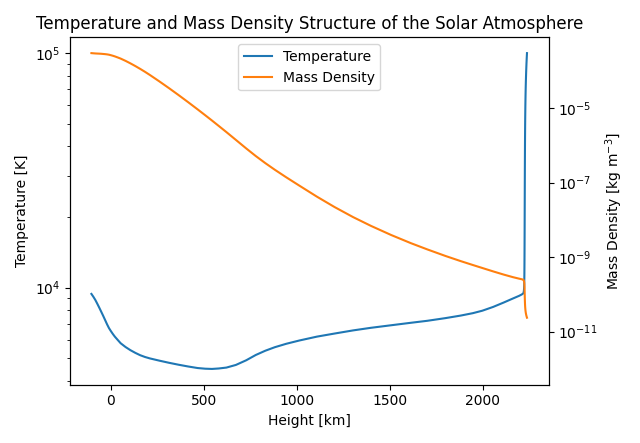
\includegraphics[width=.7\linewidth]{./00Introduction/figs/atmosphere.png}
    \caption[The temperature and pressure structure of the solar atmosphere from the model of \cite{fontenla_energy_1993}]{The temperature and pressure structure of the solar atmosphere from the model of \cite{fontenla_energy_1993}.}
    \label{atmos}
\end{figure}
The temperature and pressure structure of the solar atmosphere up to the base of the transition region can be seen in \fig{atmos}. Meanwhile the layers of the atmosphere can be seen in \fig{layers}. Suspended in the corona are the structures on which this thesis is focused: solar filaments and prominences.
\begin{figure}
    \centering
    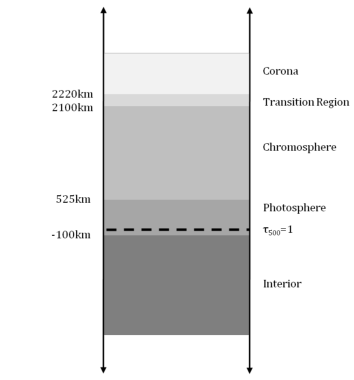
\includegraphics[width=.5\linewidth]{./00Introduction/figs/layers.pdf}
    \caption[A simplified schematic of the Solar atmosphere. Adapted from \cite{carroll_introduction_2007}]{A simplified schematic of the Solar atmosphere. Adapted from \cite{carroll_introduction_2007}.}
    \label{layers}
\end{figure}

\section{Solar Prominences and Filaments}

Solar prominences and filaments are different sides of the same coin. When viewed on disc, they are seen as dark filamentary absorption features and are called filaments. When viewed off-limb, they are seen in emission and called prominences. This distinction is due historical reasons; it was unclear that these structures were one and the same. \fig{both} shows a prominence eruption observation by the Sun-Earth Connection Coronal and Heliospheric Imager \citep[SECCHI; ][]{howard_sun_2008} onboard the Solar Terrestrial Relations Observatory Ahead \citep{driesman_stereo_2008} where it appears both in emission and absorption. The oldest reference to the observation of solar prominences comes from astronomical records in the Russian Chronicles \citep{tandberg-hanssen_solar_1974}. This is the previously mentioned observation made by Lavrentievsky in 1185. These `hot charcoals' to which he refers were very likely solar prominences. Later in 1239, Muratori observed the corona during a solar eclipse and described the corona as having a `burning hole' in it \citep[see ][]{secchi_soleil_1875}. This is also believed to have been a solar prominence \citep{tandberg-hanssen_solar_1974}. It was not until the mid-ninteenth century that serious scientific endeavour was directed towards their study. 
\begin{figure}
    \centering
    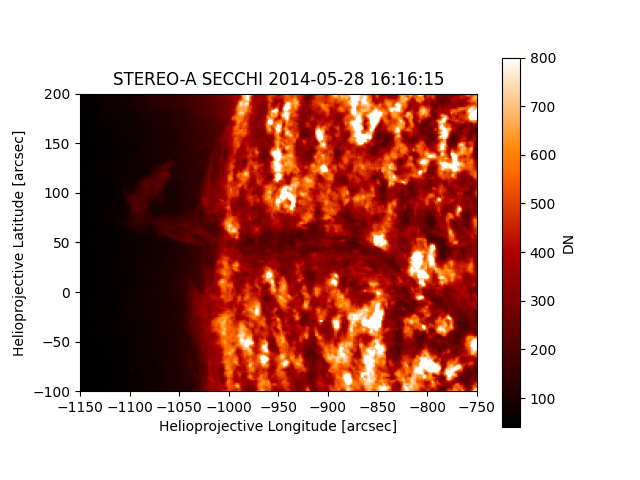
\includegraphics[width=0.7\linewidth]{./00Introduction/figs/prom.png}
    \caption[Prominence observed by the 304~\AA{} filter of STEREO-A/SECCHI]{Prominence observed by the 304~\AA{} filter of STEREO-A/SECCHI. It appears both in emission and absorption. This highlights the similarity and differences between a filament and a prominence.}
    \label{both}
\end{figure}
\subsection{Classification}
There are a number of schemes in which to classify solar prominences. These are based on their morphology, dynamic properties, and general location. Early astronomers realised that prominences in close proximity to active regions were seen to change very rapidly compared to those located in regions of the quiet Sun \citep{vial_solar_2015}. \cite{secchi_soleil_1875} divided solar prominences into three classes; the first two of which we now describe as quiescent and active prominences \citep{tandberg-hanssen_nature_1995}. The third class seems to be a description of what we now know as coronal rain, and the author retracts this third definition later in the text. \cite{secchi_soleil_1875} describes quiescent prominences as peaceful and tranquil. This is a very apt definition. Quiescent prominences tend to form in regions of the quiet Sun away from active regions. They show few motions and only show small changes over hours and/or days. These are very stable and persists from days to weeks. Additionally they are unlikely to erupt unless there is some trigger nearby, such as a flare or CME. This, however, does not mean that they are not dynamic, they are just less so than their counterparts. Active prominences tend to form in active regions and are less stable and far more dynamic than their calmer siblings. Due to the greater magnetic field in the active regions where they form, they tend to be much smaller and shorter lived. They are much more prone to spontaneous eruption than their siblings.Secchi goes on to further subdivide these main classes into subclasses comprising of clouds, filaments, stems, plumes, horns, cyclones, flames, jets, sheafs, and spikes. Presently the distinction between these subclasses is not clear and the main two categories are instead used without these subclasses.

\subsection{Formation}

There are two leading ideas about how prominences form. On one hand, many believe that some prominences form due to condensation of hot material from the corona. This approach is applied to both active and quiescent prominences. On the other hand, some prominences are believed to have photospheric or chromospheric origins, with active prominences being lifted up and out of these layers \citep{tandberg-hanssen_nature_1995}. However, all prominences form in filament channels which form around polarity inversion lines \citep[PILs; ][]{vial_solar_2015} -- regions where the photospheric magnetic field flips polarity. A filament channel forms when chromospheric fibrils align themselves with the PIL. Additionally, prominences can only form in these regions where no fibrils cross the PIL \citep{martin_conditions_1998}. The mechanism which causes these fibrils to align themselves with the polarity inversion line is not well understood and many processes to describe this phenomena have been suggested. One such suggestion is that of the submergence and cancellation of the transverse magnetic field component, leaving the axial field component behind \citep{martin_conditions_1998, wang_formation_2007}. Alternatively, it has been suggested that strong shearing motions in the photospheric plasma localised to the PIL are responsible \citep{devore_dynamical_2000}. The former may be supported by \cite{wang_transient_2013}, where they observed transient brightenings along a filament channel, which they suggest are associated with flux cancellation. The latter was explored by \cite{hindman_helioseismically_2006} where sheared flows of the order of 30\kms{} were observed to either side of a PIL. Filament channels often form with magnetic arcades, closed field lines which pass high and over the channel, anchored in regions of opposing polarity on either side of the channel. When a prominence forms in the channel, this arcade is seen to exist above both. Between the prominence and the arcade one can observe a dark coronal cavity \citep{tandberg-hanssen_nature_1995}.

\subsection{Main Components}
Prominence are seen to have two main observable features, their horizontal spine which is suspended above the solar surface, and barbs which anchor the spine to the solar surface. Barbs are very easily seen in coronal filters, such as 171~\AA{} from the Atmospheric Imaging Assembly \citep[AIA; ][]{lemen_atmospheric_2012} onboard the Solar Dynamics Observatory \citep[SDO;][see \fig{threestages}]{pesnell_solar_2012}. These features are more readily identifiable as filaments on the disc as their orientation lends well to being observed.
Another important feature of a prominence is the prominence to corona transition region \citep[PCTR; ][]{vial_solar_2015}. This is analogous to the transition region (TR) of the classic view of the solar atmosphere. Here the prominence transitions from cool photospheric and chromospheric temperatures ($\sim6000$~K) to that of coronal temperatures ($>500~000$~K). Additionally the PCTR also includes a pressure gradient (like the TR) to smoothly transition from a high pressure prominence to the more tenuous corona. As such prominences are seen to emit spectral lines of a wide range of elements. Prominences are known to be primarily composed of hydrogen and are routinely observed in H$\alpha$, with many stations around the world observing the Sun in this wavelength daily\footnote{such as https://bass2000.obspm.fr or https://gong2.nso.edu}. However, we can also observe line profiles which form at much higher temperatures, such as \mgiihk, which is the main focus of this work. This temperature and pressure gradient makes solar prominences appear more extended in ultraviolet compared to H$\alpha$ \citep{heinzel_why_2001}. When the PCTR is taken into account when modelling solar prominences, we find that we achieve a better match between observed and synthetic spectra \sectp{Chap:prom} which highlights the impact that it has on line formation in the prominence.

\subsection{Thermodynamics and General Properties}


Prominences are comprised of cool dense plasma suspended in the hot and tenuous solar corona \citep{labrosse_physics_2010}. Due to their structure, as discussed in the previous section, it is easy to see that prominences comprise of a wide range of temperatures and pressures. The core of a prominence tends to be the coolest part of the prominence, with temperatures of the order of $10^4$~K. However, the PCTR reaches much higher temperatures, of the order of $10^4-10^6$~K. The densities observed show the inverse of this, as one familiar with the TR would expect. The core of a prominence has electron densities between $10^9-10^11$~cm$^{-3}$, but this drops to $10^6-10^8$~cm$^{-3}$ in the PCTR. Pressures show a similar story with the core exhibiting pressures of the order of $0.02-1$~dyn~cm$^{-2}$ and the PCTR with $0.2$~dyn~cm$^{-2}$. It is possible for the PCTR to experience higher pressures than some internal pressures. Along with their thermodynamic properties, they also exhibit a range of motions. Fine motions within the prominence itself can be of the order of $3-20$\kms{} in the core of the prominence, up to 30\kms{}. These `microturbulent' velocities are responsible for widening the line profiles we observe from prominences. However, these are not bulk flows that can be observed directly and must be inferred from the line profiles. Bulk flows tend to be much smaller, reaching 5\kms{} in the core of the prominence and 10\kms{} in the PCTR \citep{labrosse_physics_2010}. When these flows move away from the solar surface, the radiation is subject to Doppler dimming. Any incident radiation from the solar disc arriving at the prominence is seen to be Doppler shifted by the prominence. This causes less radiation to be absorbed and scattered as the radiation arriving at the prominence is shifted relative to the absorption profile. Line profiles will be seen to be less intense than their static counterparts. 

\subsection{Magnetic Field Strength}

The magnetic field strength of a solar prominence is difficult to determine and requires some measurement of the Stokes parameters. The Stokes parameters consist of four vectors, I, Q, U, and V. I is the intensity of the observed radiation, this does not measure polarisation. Q and U measure the linear polarisation of the light. Q and U are separated by 45\degr{} such that a better measure of the polarisation can be made. V measures the circular polarisation of the light, giving $1$ and $-1$ for fully right hand polarised and left hand polarised light, respectively \citep{toro_iniesta_introduction_2007}.
The magnetic field in a prominence is typically quoted as being on the order of 1s to 10s of Gauss \citep{tandberg-hanssen_nature_1995}. Quiescent prominences have been measured to have magnetic fields of $3-15$~G, while active prominences have been observed with magnetic fields of $30-45$~G \citep{mackay_physics_2010}.



\subsection{Eruptions and Demise}

Prominences boast a range of lifetimes. This depends on whether it is a quiescent or active prominence.
It is generally accepted that instabilities lead to the demise of prominences. The source of these instabilities, however, is debated. There are two main equilibria responsible for the stability of solar prominences; thermal equilibrium and magnetohydrostatic equilibrium \citep{tandberg-hanssen_nature_1995}. The breakdown of either of these will lead to the death of a prominence. One of the more dramatic of these, is a prominence eruption. This is the expulsion of a prominence from the Sun. The most energetic of these %which reach the solar escape velocity ($v_{esc}=617.7$\kms)
are called flare sprays \citep{tandberg-hanssen_solar_1974} and are closely related to coronal mass ejections (CMEs). Prominence cores are frequently viewed as the central core of a CME in white light coronagraphs \citep{vial_solar_2015}. One model which attempts to explain the eruption of solar prominences is that of mass draining by \cite{jenkins_modeling_2019}. The authors argued that mass draining causes an instability which leads to a rise in height of the prominence. This height increase then continues until the prominence erupts or becomes completely devoid of material through draining. Which of these two fates the prominence meets depend on the conditions it is under before the draining commences. \cite{wang_transient_2013} observed brightenings at the end points of erupting filament channels in the 195~\AA{} filter of the Extreme-Ultraviolet Imaging Telescope \citep[EIT; ][]{delaboudiniere_eit_1995} onboard the Solar and Heliospheric Observatory \citep[SOHO; ][]{domingo_soho_1995}. These were interpreted to be sites of magnetic reconnection catalysed by the rise of the host magnetic field lines host to the prominence. This rise is then said to have crossed into the overlying coronal loops and reconnected with them, further accelerating the eruption via the breakdown of magnetohydrostatic equilibrium. When a quiescent prominence erupts, the source filament channel remains. This can then go on to have another prominence form in the vacant channel, starting the whole process again \citep{vial_solar_2015}. If the thermal equilibrium breaks down, the prominence can quickly heat up to coronal temperatures and effectively evaporate. Prominences lose energy by radiation, since radiative losses are proportional to the square of the density, this shows that it is an effective way to quickly dissipate radiation. If the thermal losses are too small, however, the prominence will quickly heat up. This breakdown and heating of the prominences happens on the order of seconds to minutes \citep{tandberg-hanssen_nature_1995}.

\section{Magnesium}
Magnesium is one of the most abundant elements in the solar atmosphere. Therefore its singly ionised state, \mgii{}, has great diagnostic potential \citep{leenaarts_formation_2013-1}. It is clear that once ionised magnesium, \mgii{}, is a very important ion. Its principle transitions, \mgiihk{}, form in the upper chromosphere and lower transition region \citep{depontieu_interface_2014}. This formation region will capture the hotter parts of the prominence, and gives us insight into the nature of the PCTR. The rest wavelengths of the \mgiihk{} lines are 2803.53~\AA{} and 2796.35~\AA, respectively \citep{levens_modelling_2019}. The features of the \mgiihk{} lines are usually separated into five distinct features per line. The violet features $1_\text{v}$ and $2_\text{v}$ are the points at which the wings of the emission start to increase, and when its peak violet intensity is reached, respectively. The red features, $1_\text{r}$ and $2_\text{r}$, are described similarly.
\begin{figure}
    \centering
    \includegraphics*[width=0.8\linewidth]{./00Introduction/figs/mgii.png}
    \caption{The spectral features of the \mgiihk{} lines. This spectrum was taken from the edge of the solar disc on 2018-04-19.}
    \label{fig:mgiifeatures}
\end{figure}
However, the feature labelled $3$ in \fig{fig:mgiifeatures} is the central reversal and line core. In general, the optical thickness of \mgiihk{} is such that many of its observed line profiles exhibit a central reversal. This is encapsulated by Eq. \ref{eq:line}; $\tau_\lambda$ is a function of wavelength, and in the case of \mgiihk{} $\tau_\lambda$ is largest towards the line core, and it is lowest towards the wings. This means that the line core tells us more about the surface of the plasma, but the wings allow us to see deeper into the structure. This is also the reason for the appearance of this double peak. However, there needs to be a sufficient amount of material to absorb enough of the line core for the line to manifest with a self reversal. This is because $\tau_\lambda$ is also a function of distance through the material. In solar prominences, in general we do not see this double peaked behaviour. When a line presents itself in this single peaked fashion, the $2_v$ and $2_r$ features are not present. It was shown by \cite{heinzel_formation_2014} that the \mgiihk{} line cores are very sensitive to the temperature structure in the PCTR, highlighting their diagnostic potential to explore this region. 


\section{A Brief Foray into Radiative Transfer}
Radiative Transfer is the study of how electromagnetic radiation moves through and interacts with a medium. As put by \cite{hubeny_theory_2015}, `The radiation we receive from a star contains an enormous wealth of information about the structure and composition of its atmosphere.' This should be motivation enough on its own to study this extremely interesting field. Disregarding magnetic complexities, there are  five main processes which govern the solar spectra that we observe; bound-free (bf) interactions, where atoms are ionised and recombine liberating a photon in the process; free-free (ff) interactions, where electrons collide with ionised nuclei causing a photon to be emitted due to the energy lost by the electron; bound-bound (bb) interactions, where electrons move from one energy level to another within the same atom; and Rayleigh and Thomson scattering, where the former concerns photons scattering from neutral hydrogen, and the latter, photons scattering from free electrons \citep{rutten_introduction_1993}. The radiation received from an emitting medium can be represented by the specific intensity,
\begin{equation}
    \frac{\dd I_\lambda}{\dd s}=j_\lambda-\chi_\lambda I_\lambda,
    \label{eq:1}
\end{equation}
where $j_\lambda$ is the monochromatic emissivity, $\chi_\lambda$ is the linear extinction coefficient, and $s$ is the path length of the beam. Kirchoff's Law which defines the source function $S_\lambda$ is also important \citep{woan_cambridge_2000},
\begin{equation}
    S_\lambda\equiv\frac{j_\lambda}{\chi_\lambda}.
\end{equation}
This describes the energy of new photons entering the beam, and is normalised by the linear extinction coefficient which describes the extinction of the radiation as it travels through the medium. $\chi_\lambda$ is related to the optical path length by,
\begin{equation}
    \dd\tau_\lambda(s)=\chi_\lambda(s)\dd s.
    \label{eq:3}
\end{equation}
This allows us to define the optical thickness as,
\begin{equation}
    \tau_\lambda(D)=\int_0^D\chi_\lambda(s)\dd s,
\end{equation}
where $D$ is the path length through the material. Combining Eqs. \ref{eq:1} and \ref{eq:3} allows us to change variables from $s$ to $\tau_\lambda$ such that,
\begin{equation}
    \frac{\dd I_\lambda}{\dd \tau_\lambda}=S_\lambda-I_\lambda.
\end{equation}
Then multiplying through by $\exp(\tau_\lambda(D))$ and integrating between 0 and $\tau_\lambda(D)$ we get,
\begin{equation}
    I_\lambda(\tau_\lambda)=I_\lambda(0)\exp(-\tau_\lambda)+\int_0^{\tau_\lambda}S_\lambda(t_\lambda)\exp(-(\tau_\lambda-t_\lambda))\dd t_\lambda.
\end{equation}
$\tau_\lambda$ is implicitly a function of distance here. $t_\lambda$ describes the path length in terms of optical depth. If we assume that the source function is constant across $t_\lambda$, we can evaluate this integral and change variables such that,
\begin{equation}
    I_\lambda(D)=I_\lambda(0)\exp(-\tau_\lambda)+
    \overline{S_\lambda}\left(1-\exp\left(-\tau_\lambda\right)\right),
    \label{eq:line}
\end{equation}
and what we have is the formal solution to the radiative transfer equation. $I_\lambda(0)$ is the radiation entering the material, and $\overline{S_\lambda}\left(1-\exp\left(-\tau_\lambda\right)\right)$ describes the radiation created by the material that can reach $D$, and $I_\lambda(D)$ is the total radiation at $D$ given that $\tau_\lambda=\tau_\lambda(D)$. In local thermodynamic equilibrium (LTE) the source function becomes the Planck function, $B_\lambda$, such that \citep{rutten_introduction_1993,hubeny_theory_2015},
\begin{equation}
    I_\lambda(D)=I_\lambda(0)\exp(-\tau_\lambda)+
    B_\lambda\left(1-\exp\left(-\tau_\lambda\right)\right).
\end{equation}
If there is a coherent and isotropic scattering term, the source function is modified to become \citep{hubeny_theory_2015}, 
\begin{equation}
    S_\lambda=\epsilon_\lambda B_\lambda+(1-\epsilon_\lambda)J_\lambda,
\end{equation}
where $\epsilon$ is the thermal coupling parameter or destruction probability, and $J_\lambda$ is the mean intensity of radiation, ie the mean of the specific intensity over all solid angles. If the reader wishes, $\lambda$ may be substituted for $\nu$ in any of these equations.
This powerful set of equations can help us to model the radiation that comes from the solar atmosphere to better understand how the radiation we see from the Sun is formed.

For a simple 2-level atom, the source function takes the form of \citep{hubeny_theory_2015,levens_diagnostics_2018},
\begin{equation}
    S_{lu}=\frac{n_uA_{ul}}{n_lB_{lu}-n_uB_{ul}}\frac{\psi_{ul}(\lambda)}{\phi_{lu}(\lambda)}
\end{equation}
Where $A$ and $B$ are the Einstein coefficients. $A_{ul}$ denotes spontaneous emission, $B_{ul}$ denotes stimulated emission, and $B_{lu}$ denotes absorption. $n_u$ is the population of the upper level, $n_l$ is the population of the lower level. $\psi_{ul}(\lambda)$ is the emission profile and ${\phi_{lu}(\lambda)}$ is the absorption profile. In complete redistribution (CRD), it assumed that there are enough collisions in the plasma such that when a photon is absorbed by an atom, the atom relaxes such that the photon is re-emitted anywhere in the line. That is to say, that $\psi_{ul}(\lambda)$=${\phi_{lu}(\lambda)}$. On the opposite end of this is scattering, where an absorbed photon is re-emitted at its original wavelength and its not redistributed along the line. Partial redistribution (PRD) is a combination of these two regimes. The photon is more likely to be re-emitted at a small range of frequencies around its original frequency. In the CRD approximation, the source function becomes,
\begin{equation}
    S_{lu}\approx\frac{n_uA_{ul}}{n_lB_{lu}-n_uB_{ul}}
\end{equation}
However, as shown by \cite{milkey_resonance_1974}, this does not hold in the optically thick regime. This includes ions such as \mgii. Under non-LTE conditions, the source function varies from the Planck function. This cannot be solved analytically and must be solved numerically. This is because the source function is strongly dependent on the radiation field \citep{labrosse_physics_2010}. Careful consideration of the level populations and radiation field is required to find the source function. The equations of statistical equilibrium are used to achieve this \citep{labrosse_physics_2010},
\begin{equation}
    \frac{dn_i}{dt}=\sum_{j\neq i} n_j\left(R_{ji}+C_{ji}\right)-n_i\sum_{j\neq i} \left(R_{ij}+C_{ij}\right)
\end{equation}
\begin{equation}
    \frac{dn_i}{dt}=\frac{\partial n_i}{\partial t}+\frac{\partial n_iV}{\partial x}
\end{equation}
Like before, $n_i$ is the population of the ith level, and $n_j$ is the population of the jth level. V is the flow velocity. $C_{ij}$ and $C_{ji}$ are the collisional rates which are proportional to the electron density ($n_e$). $R_{ij}$ and $R_{ji}$ are the radiative rates for absorption and stimulated emission. These depend on the radiation field of the line and continuum.  For a simple two level atom like before, the equations of statistical equilibrium can be simply written as \citep[ignoring the time and velocity terms,][]{labrosse_physics_2010},
\begin{equation}
    n_lB_{lu}\overline{J}_{lu}+n_lC_{lu}=n_uA_{ul}+n_uB_{ul}\overline{J}_{lu}+n_uC_{ul}
\end{equation}

\section{Radiative Transfer Code}

Recently, there has been 3D prominence modelling efforts by \citep{gunar_3d_2015}. They employ, what they name, 3D whole-prominence fine structure (WPFS) modelling. Where they model a 3D magnetic field using the 3D non-linear force-free (NLFF) simulations of \cite{mackay_non-linear_2009}, in which they identify dips or hammocks which they then allow to fill with plasma. This geometry is then used as the configuration for radiative transfer simulations. The study shows the importance of the projection effect and naturally reproduces fine structure emission. While this method is very powerful, the authors have little control over the geometry of the simulation like we do in more conventional approaches. Both methods have their pros and cons, but this WPFS modelling is still quite new with a lot of potential. While it is possible to use it to simulate a prominence if we know the underlying magnetic field, it may also be possible to infer the magnetic field structure if we start with an observation of a prominence and work backwards. 

In this thesis, we use two radiative transfer codes to solve them numerically. We first introduce the 1D non-local thermodynamic equilibrium (NLTE) RT code, PROM. Later introducing the 2D NLTE RT code, RTCY.

\subsection{PROM}
\label{promintro}
\begin{figure}
    \centering
    \includegraphics*[]{./02Modelling1D/figs/20180419/prom.png}
    \caption[Construction of the simulation in PROM. Based on \cite{gouttebroze_formation_1997} and \cite{labrosse_effect_2007}.]{Construction of the simulation in PROM. The curvature of the Sun is exaggerated in this cartoon. Based on \cite{gouttebroze_formation_1997} and \cite{labrosse_effect_2007}.}
    \label{promsetup}
\end{figure}
\cite{gouttebroze_hydrogen_1993} and \cite{heinzel_theoretical_1994} introduced the 1D radiative transfer code, PROM. PROM solves the set of radiative transfer equations to produce symmetrical (around the line core) line profiles. In its initial implementation, it only produced hydrogen spectra. The lines exhibited in \cite{gouttebroze_hydrogen_1993} were Ly$\alpha$, Ly$\beta$, H$\alpha$, Ly$\gamma$, H$\beta$, and P$\alpha$ -- the first six bound-bound neutral hydrogen transitions. In theory, any bound-bound line produced by a twenty level hydrogen atom could be output from PROM. Additionally, the bound-free transition of the Lyman continuum is included. This aimed to improve on the work by \cite{heasley_theoretical_1974} where the authors adapted NLTE code to the problem of an illuminated slab/prominence. Throughout the years, many modifications have been made to PROM; \cite{gouttebroze_formation_1997} and \cite{gouttebroze_calcium_2002} introduced the \ion{Ca}{ii} lines. Here, a five level \ion{Ca}{ii} ion is implemented, with an additional level for unionised (\ion{Ca}{i}) and twice ionised (\ion{Ca}{iii}), respectively. This allowed for the modelling of the \ion{Ca}{ii}~H\&K lines. \cite{labrosse_formation_2001} introduced the \ion{He}{i} and \ion{He}{ii} lines, with a 33 level (plus continuum) atom for both \ion{He}{i} and \ion{He}{ii}. \cite{labrosse_nonlte_2004} introduced the prominence-to-corona transition region (PCTR) as formulated in \cite{anzer_energy_1999}. The PCTR takes the form of a pressure ($p$) and temperature ($T$) gradient as a function of column mass, $m$. 
\begin{equation} 
    T(m)=T_{\text{cen}}+(T_{\text{tr}}-T_{\text{cen}})\left(1-4\frac{m}{M}\left(1-\frac{m}{M}\right)\right)^\gamma
    \label{tstrat}
\end{equation}
\begin{equation}
    p(m)=4p_c\frac{m}{M}\left(1-\frac{m}{M}\right)+p_{\text{tr}},
    \label{pstrat}
\end{equation}
where,
\begin{equation}
    p_c=\frac{{B_{z_0}}^2}{8\pi}=p_{\text{cen}}-p_{\text{tr}},
    \label{pcdef}
\end{equation}

where $M$ is the total column mass, $\frac{M}{2}$ is the centre of the prominence, $B_{z_0}$ is magnetic field perpendicular to the solar surface, $T_{\text{cen}}$ and $p_{\text{cen}}$ are the central temperature and pressure respectively, and $T_{\text{tr}}$ and $p_{\text{tr}}$ are the temperature and pressure at the outer edge of the PCTR respectively. These equations \citep{anzer_prominence_1998, anzer_energy_1999,labrosse_nonlte_2004} allow the core of the prominence to gently transition to the corona without discontinuity. The value of $\gamma$ is strictly more than 0. If $\gamma=0$, the prominence becomes isothermal with a temperature of that of the corona, while the pressure still gradually changes. A prominence of such conditions is not possible in nature. \cite{levens_modelling_2019} builds on the \ion{Ca}{ii} formulation from \cite{gouttebroze_formation_1997} to introduce a five level (plus continuum) \mgii{} ion to produce the \ion{Mg}{ii}~h\&k lines (2803.53~\AA\ and 2796.35~\AA) and the \ion{Mg}{ii} triplet lines (2791.60~\AA, 2798.75~\AA, and 2798.82~\AA). When modelling these lines, it must be considered whether CRD or PRD is used.  It was shown by \cite{milkey_resonance_1974} that PRD is important when modelling the \mgii{} resonance lines, and so partial redistribution (PRD) is used here. The incident \mgii{} radiation is taken from near disc centre spectroscopic \ion{Mg}{ii} observations from the Interface Region Imaging Spectrograph \citep[IRIS;][]{depontieu_interface_2014}.
\begin{figure}
    \centering
    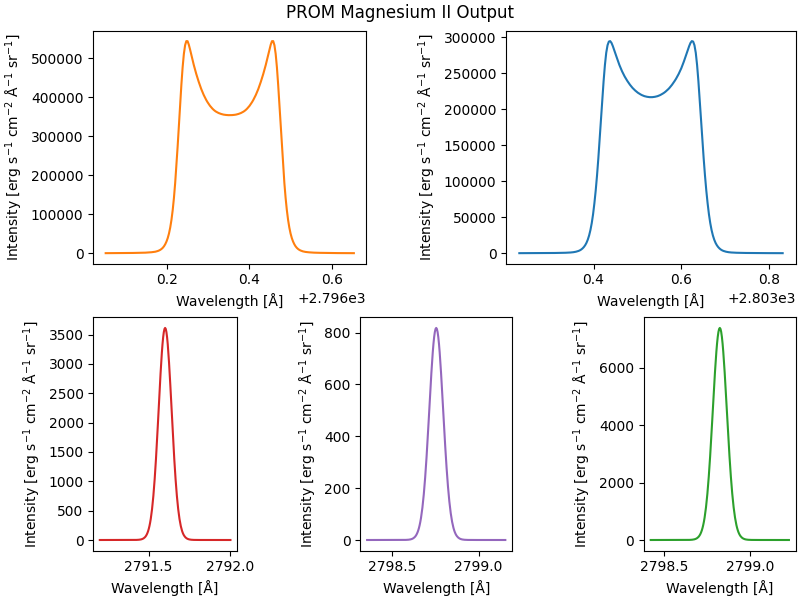
\includegraphics[width=0.9\linewidth]{./02Modelling1D/figs/20180419/promexample2.png}
    \caption[An example of the magnesium output from PROM.]{An example of the magnesium output from PROM. The top panels are \mgiihk{}, respectively, while the bottom panels are the \mgii{} triplet lines. The parameters of this model are; $T_\text{cen}=8000~$K, $T_\text{tr}=100000~$K, $p_\text{c}=0.5~$dyn$~$cm$^{-2}$, $p_\text{tr}=0.01~$dyn$~$cm$^{-2}$, $\gamma=5$, $v_T=5~$km$~$s$^{-1}$, $H=10~$Mm, and $v_{rad}=0~$km$~$s$^{-1}$.}
    \label{promexample}
\end{figure}

Within PROM, prominences are represented by a semi-infinite plane parallel slab perpendicular to the solar surface. This slab is illuminated on both sides by the angle-averaged incident intensity. A schematic diagram can be seen in Fig. \ref{promsetup}. PROM (with a PCTR) has several input parameters. surface temperature, the temperature at the edge of the PCTR ($T_{\text{tr}}$ in \eq{tstrat}); central temperature, the temperature in the core of the prominence ($T_{\text{cen}}$ in \eq{tstrat}); surface pressure, the pressure at the edge of the PCTR ($p_{\text{tr}}$ in \eq{pstrat}); central gas pressure, the central gas temperature of the prominence ($p_{\text{c}}$ in eqs. \ref{pstrat} and \ref{pcdef}); thickness, the geometric width of the prominence along the line of sight ($L$ in Fig. \ref{promsetup}); column mass, the mass as a function of distance through the prominence; $\gamma$, a dimensionless number which dictates the extent of the PCTR; microturbulent velocity, the unresolved stochastic motions within the prominence; altitude, the height above the solar surface ($H$ in Fig. \ref{promsetup}); and radial velocity, bulk velocity away (when positive) or towards (when negative) from the Solar surface ($v_\text{rad}$ in Fig. \ref{promsetup}). The outputs are the intensities of the considered line profiles, the number density of the considered species, their level populations, and the optical thickness of the line core. An example of the \mgii\ line profiles output from a run of PROM from \cite{levens_modelling_2019} can be seen in Fig. \ref{promexample}. The spectral resolution of these simulated line profiles is 3~m\AA, much greater than any current instrument.

\subsection{RTCY}
\label{rtcyintro}
Radiatif Transfert Cylindrique (Cylindrical Radiative Transfer; RTCY) was developed over a series of seven papers \citep{gouttebroze_radiative_2004,gouttebroze_radiative_2005,gouttebroze_radiative_2006,gouttebroze_radiative_2007, gouttebroze_radiative_2008, gouttebroze_radiative_2009,labrosse_radiative_2016}. The prominence is modelled as a cylinder suspended above the solar surface with a set of thermodynamic, geometric, and dynamic properties. Currently, this model is isobaric. However, it is possible to include a PCTR for the temperature gradient. The implementation of the geometric and dynamic properties can be seen in \fig{fig:rtcyv5}. 
\begin{figure}
    \centering
    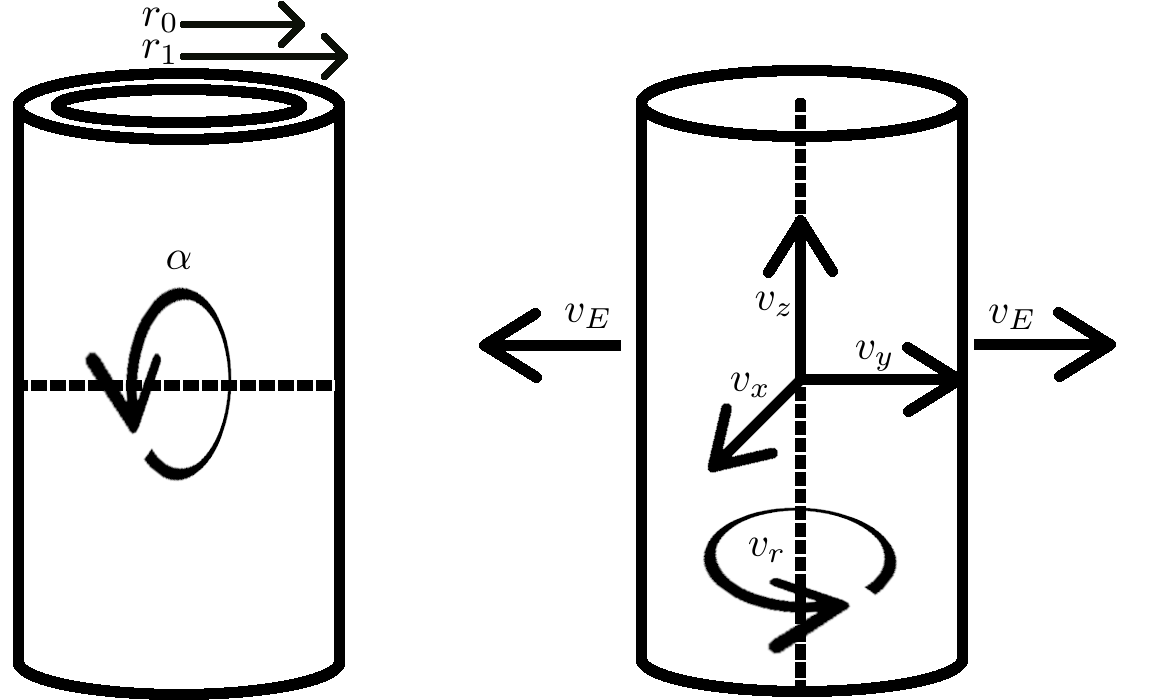
\includegraphics[width=0.71\linewidth]{./03Modelling2D/figs/rtcy.png}
    \caption[The prominence model employed by RTCY.]{The prominence model employed by RTCY. The observer is looking from the right to the left and the Solar surface is parallel to the bottom of the page. \textit{Left}: The geometric properties of the prominence model.  \textit{Right}: The velocity settings of the model. The $v_E$ arrows should be placed all around the circumference of the cylinder, but are omitted for clarity. Please note that $x$ is out of the page.}
    \label{fig:rtcyv5}
\end{figure}
\begin{figure}
    \centering
    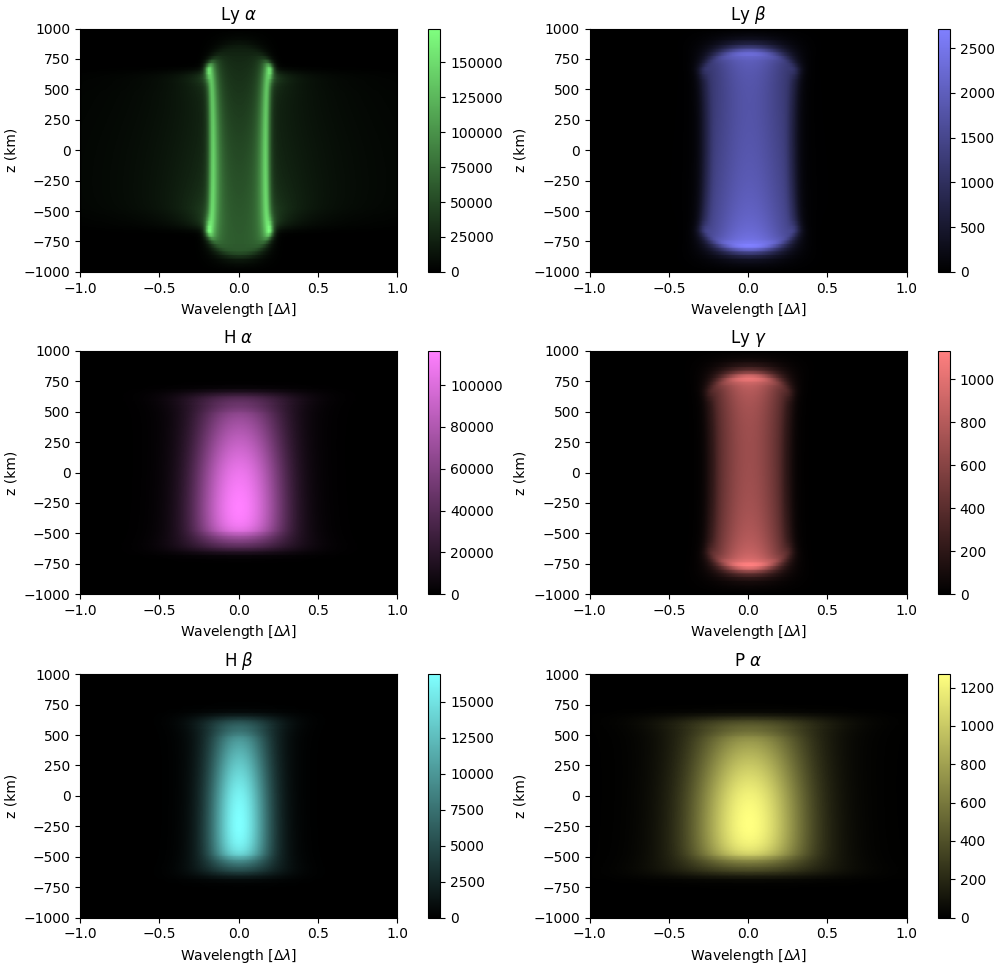
\includegraphics[width=\linewidth]{./03Modelling2D/figs/exh.png}
    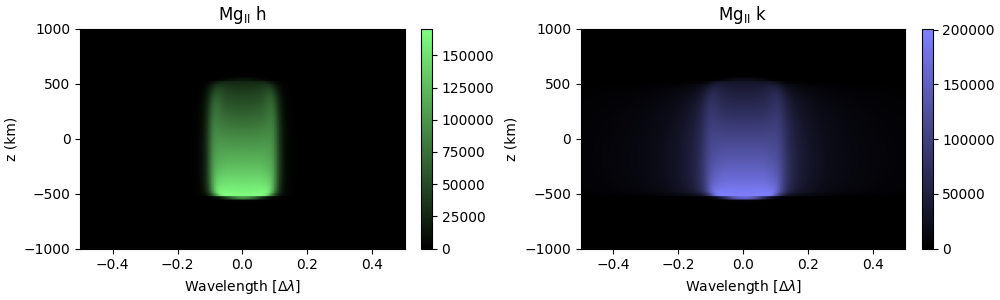
\includegraphics[width=\linewidth]{./03Modelling2D/figs/exmg.png}
    \caption[Example of the output of RTCY for the principal neutral hydrogen transitions and the h\&k lines of once-ionised magnesium.]{Example of the output of RTCY for the principal neutral hydrogen transitions and the h\&k lines of once-ionised magnesium. The units of the colourbars are \cgsint. The parameters of this example run are; $P=0.1$~dyn~cm$^{-2}$, $r_0=500$~km, $r_1=1000$~km, $T_0=6000$~K, $T_1=100~000$~K, $v_T=5$~km~s$^{-1}$, $\alpha=\frac{\pi}{2}$~rad and $H=10000$~km with no velocity setting active.}
    \label{fig:introexhmg}
\end{figure}
For the geometric properties, $r_0$ is the radius for which the cylinder is isothermal in km; $r_1$ is the radius of the PCTR in km; and $\alpha$ is the rotation of the cylinder, where $\alpha\in[0,\frac{\pi}{2}]$ due to symmetry. Not included on this diagram is $H$, the height above the solar surface in km. 
The thermodynamic properties include the gas pressure ($P$) in dyn~cm$^{-2}$; temperature in the core of the prominence ($T_0$) in K; temperature of the PCTR ($T_1$) in K; and the microturbulent velocity within the prominence ($v_T$) in km~s$^{-1}$. RTCY also has an isothermal and isobaric mode, where $T_0$ and $T_1$ are replaced by a single temperature, $T$, and $r_0$ and $r_1$ are replaced by a single diameter, $D$.
There are three main velocity settings; $v_x$, $v_y$, and $v_z$ which make up the translation velocity setting in km~s$^{-1}$; $v_E$ is the expansion velocity setting in km~s$^{-1}$ where the whole prominence expands radially outward from the axis of rotational symmetry; and $v_r$ is the rotational velocity setting in rad~s$^{-1}$. These settings can only be run independently of one another due to the way velocities are currently implemented. If more than one of these is specified in the run parameters, the expansion velocity setting takes precedence, followed by the rotational velocity setting, and finally the translational velocity setting has the lowest precedence. 
The code simulates the emission that would be seen by a single slit of a hypothetical spectrometer aligned along $z$. The version of the code employed here simulates hydrogen and magnesium emission. By default, it produces the Ly$\alpha$, Ly$\beta$, H$\alpha$, Ly$\gamma$, H$\beta$, P$\alpha$; and \mgii{}~h and \mgii{}~k lines. This code uses Complete Redistribution (CRD) for these resonance lines. See \fig{fig:exhmg} for an example of the output of the code. The parameters of this example run were; $P=0.1$~dyn~cm$^{-2}$, $r_0=500$~km, $r_1=1000$~km, $T_0=6000$~K, $T_1=100~000$~K, $v_T=5$~km~s$^{-1}$, $\alpha=\frac{\pi}{2}$~rad and $H=10000$~km with no velocity setting active. Although RTCY produces hydrogen spectra, here we focus on the \mgiihk{} spectra.
To visualise the output of RTCY a secondary code, named cbaem, is used to generate encapsulated postscript (eps) and portable document format (pdf) figures identical to that seen in \fig{fig:introexhmg}. However, cbaem was rewritten in Python3 in order to pull out extra information about the plasma conditions, such as the optical depth, such that plots similar to Figs 4 through 7 of \cite{carlsson_formation_1997} could be produced for these prominence simulations \chapp{Chap:2DModel}


\section{Instrumentation}
The main instrument used is the space based Interface Region Imaging Spectrograph \citep[IRIS; ][]{depontieu_interface_2014} satellite. Observations also include data from the Atmospheric Imaging Assembly \citep[AIA; ][]{lemen_atmospheric_2012} onboard the Solar Dynamics Observatory \citep[SDO; ][]{pesnell_solar_2012}; the X-Ray Telescope \citep[XRT; ][]{golub_x-ray_2007} instrument onboard the Hinode \citep{kosugi_hinode_2007} satellite; the Sun-Earth Connection Coronal and Heliospheric Imager \citep[SECCHI; ][]{howard_sun_2008} on board the Solar Terrestrial Relations Observatory Ahead \citep[STEREO-A; ][]{driesman_stereo_2008} and \ha{} observations from the Observatoire de Meudon in Paris, France. The following sections outline the capabilities of these instruments. Data from these instruments are reduced and analysed through the use of both Python and the Interactive Data Language (IDL) and the SolarSoft (SSW) library written for and in IDL \citep{freeland_data_1998}.


\subsection{The Interface Region Imaging Telescope}
The Interface Region Imaging Telescope \citep[IRIS; ][]{depontieu_interface_2014} is a NASA small explorer mission developed and operated by the Lockheed Martin Solar and Astrophysics Laboratory (LMSAL). The satellite was launched on the 27th June 2013 into a sun-synchronous orbit taking roughly 98 minutes to complete a full orbit. IRIS is a 19~cm Cassegrain Telescope with two instruments -- a slit spectrograph and its `slit jaw' imager (SJI). The latter takes images that give context for the spectrograph. IRIS is designed to study the chromosphere, transition region, and corona. While many chromospheric and transition region lines are in emission from prominences, in practice, the \mgiihk{} spectrograph is the most useful. The nominal resolution along the slit of the IRIS spectrograph is 1/6~\arcsec; this can be binned to a coarser resolution to improve the signal-to-noise ratio. The slit is of length 175~\arcsec, which at 1~AU is approximately 127~Mm, and has a width of 1/6~\arcsec. The slit spectrograph has two operating modes; sit-and-stare, where the telescope is pointed at some region and observes; and rasterised mode, where the telescope takes equally-spaced slit spectra to make up an image similar to how a rolling shutter camera operates. The rasterised mode has three different options for the spacing between rasters; dense, sparse and coarse with spacings of 1/3~\arcsec, 1~\arcsec, and 2~\arcsec, respectively. Table 12 in \cite{depontieu_interface_2014} lists all 49 of the different observing modes possible with IRIS.

The orbit of IRIS causes it to pass through the South Atlantic Anomaly (SAA) where there is a dip in the magnetic field of the Earth which causes the inner Van Allen Belt to sit lower than usual. These belts contain high energy particles which strike the detector and interfere with the electronics of the satellite. Any data taken during a pass of the SAA must be carefully analysed or discarded altogether.  
\begin{table}[]
    \centering
    \begin{tabular}{|c|c|c|}
    \hline
    Filter & Principle Ion                   & Passband                                                             \\ \hline\hline
    FUV 1  & \ion{C}{ii}  & 1331.7~\AA{} -- 1358.4~\AA \\ 
    \hline
    FUV 2  & \ion{Si}{iv} & 1389.0~\AA{} -- 1407.0~\AA \\ 
    \hline
    NUV    & \mgii        & 2782.7~\AA{} -- 2834.1~\AA \\ \hline
    \end{tabular}
    \caption{The passbands of the IRIS Spectrograph.}
    \label{irisspec}
\end{table} 
\begin{table}[]
    \centering
    \begin{tabular}{|c|c|c|}
    \hline
    Filter   & Wavelength & Passband  \\ \hline\hline
    Glass    & 5000\AA      & broadband \\ \hline
    \ion{C}{ii}      & 1349\AA      & 55\AA       \\ \hline
    \mgiihk   & 2796\AA      & 4\AA        \\ \hline
    \ion{Si}{iv}     & 1390\AA      & 55\AA       \\ \hline
    \mgii{} Wing & 2830\AA      & 4\AA        \\ \hline
    Broad    & 1370\AA      & 90\AA       \\ \hline
    \end{tabular}
    \caption{The passband of the IRIS SJI.}
    \label{irissji}
\end{table}

The IRIS spectroscope has three spectral windows, the two far ultraviolet (FUV) windows, and one near ultraviolet (NUV) window.  The passbands of which can be seen in Table \ref{irisspec}. The SJI has six different passbands, three of which work in tandem with the FUV1, FUV2, and NUV filters. The other three are the glass, \mgii{} Wing and broad filters. These can take different kinds of images to support particular observations. The passbands of these filters can be seen in Table \ref{irissji}. IRIS frequently coordinates observations with Hinode, which brings us to the next instrument.

\subsection{Hinode}
The Hinode observatory \citep[formerly known as Solar-B; ][]{kosugi_hinode_2007} was launched in September 2006. It is the spiritual successor to Yohkoh  \citep[formerly known as Solar-A; ][]{ogawara_solar-mission_1991} and will be succeeded by the yet unnamed Solar-C \citep{shimizu_solar-c_euvst_2019}. Hinode is equipped with a suite of instruments. These are the Solar Optical Telescope \citep[SOT; ][]{suematsu_solar_2008}, the EUV Imaging Spectrometer \citep[EIS; ][]{culhane_euv_2007}, and the X-Ray Telescope \citep[XRT; ][]{golub_x-ray_2007}. 

SOT is a 50~cm Gregorian telescope equipped with two filtergraphs and a spectropolarimeter. It observes in the visible wavelength range of 3880-6880~\AA{} with a spatial resolution of 0.2 to 0.3~\arcsec. In the past this has produced beautiful images of prominences, but SOT is not used in this work. EIS is designed to observe the upper transition region and solar corona. This makes EIS a good complimentary instrument to observe with IRIS. EIS uses a 0.5~m diffraction limited telescope with two wavelength windows of 170-210~\AA{} and 250-290~\AA. The field of view of this instrument is 6.0~\arcmin$\times$8.5~\arcmin. Even though it is a good counterpart to IRIS, we do not use this instrument either. XRT is designed to probe the higher energy emission from the solar atmosphere with a temperature range of $6.1<\log T<7.5$. XRT uses a grazing optics focusing system. XRT has a range of aperture filter combinations, but the Al Poly/Open configuration allows us to image the coronal cavities in which prominences can exist. When combined with IRIS, this gives us good context for the configuration of the corona surrounding the prominence.

\subsection{The Solar Dynamics Observatory}

The Solar Dynamics Observatory \citep[SDO; ][]{pesnell_solar_2012} is a NASA satellite launched on the 11th February 2010 into a Sun-synchronous orbit as part of NASA's Living With Star Program and operated by the Goddard Spaceflight Center (GSFC) with goals of monitoring space weather and deepening our understanding of the Sun. SDO houses three science instruments, the Atmospheric Imaging Assembly \citep[AIA; ][]{lemen_atmospheric_2012}, the Helioseismic and Magnetic Imager \citep[HMI;][]{scherrer_helioseismic_2012}, and the Extreme Ultraviolet Variability Experiment \citep[EVE; ][]{woods_extreme_2012}.

AIA captures high resolution high cadence full disc ultraviolet (UV) images, with an image size of 4096$\times$4096 pixels, with a spatial pixel size of 0.6~\arcsec{} and a cadence of 12, 24 or 36000 seconds depending on the filter.
AIA has four 20~cm dual-channel normal incidence telescopes. The dual-channels for each of the telescopes are as follows, 131~\AA/335~\AA, 193~\AA/211~\AA, 171~\AA/UV, and 94~\AA/304~\AA, for telescopes one, two, three, and four, respectively \citep{lemen_atmospheric_2012}. All the telescopes other than telescope two rely on filter wheels to switch between filters. Telescope two uses an `aperture blade' to select its wavelength. Additionally the UV half of telescope three has a MgF$_2$ window coating centred at 1600~\AA. All of the UV filter which share the same half of one of the telescopes is why the 1600~\AA, 1700~\AA, and 4500~\AA{} filters have a slower cadence than their EUV partners. The 24 second cadence of 1600~\AA{} and 1700~\AA{} comes from having their images taken every other cycle with respect to one another. Additionally, on the hour, one of the 1700~\AA{} images is replaced by a 4500~\AA{} image.
\begin{table}[]
    \centering
    \begin{tabular}{|c|c|c|}
    \hline
    \begin{tabular}[c]{@{}c@{}}Wavelength\\ Channel (AA)\end{tabular} & Main Ion          & Temporal Resolution (s) \\ \hline
    94                                                                & \ion{Fe}{xviii}           & 12                      \\ \hline
    131                                                               & \ion{Fe}{xviii,xii}       & 12                      \\ \hline
    171                                                               & \ion{Fe}{ix}              & 12                      \\ \hline
    193                                                               & \ion{Fe}{xii,xxiv}        & 12                      \\ \hline
    211                                                               & \ion{Fe}{xiv}             & 12                      \\ \hline
    304                                                               & \ion{He}{ii}              & 12                      \\ \hline
    335                                                               & \ion{Fe}{xvi}             & 12                      \\ \hline
    1600                                                              & \ion{C}{iv} and Continuum & 24                      \\ \hline
    1700                                                              & Continuum         & 24$^a$                     \\ \hline
    4500                                                              & Continuum         & 3600                    \\ \hline
    \end{tabular}
    \caption{Wavelength Channels of AIA \citep{lemen_atmospheric_2012}. $^a$ 48 on the hour once every hour.}
    \label{aiatable}
\end{table}
Depending on the filter, different ions and layers of the atmosphere may be imaged. Table \ref{aiatable} shows the windows and the elements which they target. Most of the EUV windows are sensitive to coronal emission. However, the main contributing ion of the 304~\AA{} filter is \ion{He}{ii}. This is formed at chromospheric temperatures and strongly seen in prominences \citep{labrosse_nonlte_2004}. This demonstrates that this is a good context imager for our observations. Certain components of prominences are also visible in the coronal channels. These channels include the 171~\AA{} and 193~\AA{} filters where the prominence barb, which grounds the structure to the disc can be seen in absorption. It is also possible to see the PCTR in these filters as a shroud surrounding the barb. 

HMI is a joint project of the Stanford University Hansen Experimental Physics Laboratory, the Lockheed Martin Solar and Astrophysics Laboratory, the high Altitude Observatory, and other institutions. The project is designed to study the dynamics of the convection zone, evolution of sunspots, active regions, and other magnetic phenomena. Like AIA, it has a 4096$\times$4096 pixel camera with a spatial pixel size of 0.5~\arcsec{}, however, the cadence of its images is lower. HMI captures full-disc Doppler velocity, line-of-sight photospheric magnetic flux, and photospheric continuum proxy images every 45 seconds. Additionally, it takes vector magnetic field maps every 90 or 135 seconds. The cadence depends on the image frame sequence. These magnetic flux maps can allow us to look at the magnetic footing of solar prominences, and study how the evolving magnetic field affects their stability.


\subsection{The Solar Terrestrial Relations Observatory}

The Solar Terrestrial Relations Observatory \citep[STEREO; ][]{driesman_stereo_2008} is a pair of twin satellites, operated by NASA, launched on 26th of October 2006, which after several flybys of the Moon escaped Earth's gravity and entered into two different heliocentric orbits with orbital radii of approximately 1~AU. The twins satellites are named STEREO-A (Ahead) and STEREO-B (Behind) referring to the direction in which they orbit relative to the Earth. This gives us two separate viewpoints from two identical spacecraft, which allows us to construct stereoscopic observations from their instruments. The experiments included on the STEREO spacecraft are; the Sun-Earth Connection Coronal and Heliospheric Imager \citep[SECCHI; ][]{howard_sun_2008}; In situ Measurements of Particles and CME Transients \citep[IMPACT; ][]{luhmann_stereo_2008}; Plasma and Suprathermal Ion Composition \citep[PLASTIC; ][]{galvin_plasma_2008}; and STEREO/WAVES \citep[S/WAVES; ][]{bougeret_swaves_2008}. Unfortunately, communications with STEREO-B were lost on 1st October 2014 due to hardware anomalies. On the 21st August 2016 when communications were briefly reestablished, NASA was unable to fully recover the spacecraft and STEREO-B has been out of contact since then. Even so, we can now use the extreme ultraviolet imager (EUVI) of SECCHI on STEREO-A in combination with AIA on SDO to produce similar stereoscopic observations that were possible with the full STEREO observatory. EUVI captures high-resolution images of the whole sun, half the resolution of AIA (2048$\times$2048 pixels), at four different wavelengths. These wavelengths and their main contributing ions are listed in Table \ref{secchitable}.
\begin{table}[h]
\centering
\begin{tabular}{|c|c|}
\hline
Wavelength Channel (\AA) & \begin{tabular}[c]{@{}c@{}}Main Contributing\\ Ion\end{tabular} \\ \hline\hline
171                                                                               & Fe\textsc{ix}             \\ \hline
195                                                                               & Fe\textsc{xii}           \\ \hline
284                                                                               & Fe\textsc{xv}             \\ \hline
304                                                                               & He\textsc{ii}             \\ \hline
\end{tabular}
\caption{Wavelength Channels of SECCHI \citep{howard_sun_2008}}
\label{secchitable}
\end{table}
As with AIA, three of these are very useful for prominence observations.  Depending on its position, STEREO-A can see parts of the far side of the Sun relative to the Earth. This is useful if you wish to track a feature, such as a prominence, to the reverse side of the Sun. STEREO-A can be used to track prominences which have rotated out of the view of AIA to see if they persist or not.

\section{Concluding Remarks}
This concludes our brief overview of the instrumentation and radiative transfer which will be employed in this work to further our understanding of the structure and evolution of solar prominences. As previously stated, the main observatory that will be used is IRIS with support and context images from AIA and STEREO. The focus is on NLTE \mgiihk{} radiative transfer modelling which will be used to invert and deduce the properties of solar prominences. 